%%
%% Copyright (c) 2018 The Authors.  All Rights Reserved.
%%
%% Weitian LI, et al.
%% School of Physics and Astronomy, Shanghai Jiao Tong University,
%% Shanghai, China.
%%
%% 2018-08-23
%%

\documentclass[letters,a4paper,fleqn,usenatbib]{mnras}
%\documentclass[letters,a4paper,fleqn,usenatbib,doublespacing]{mnras}
% Available options:
% - letters : for papers in the journal's Letters section (<=5 pages)
% - onecolumn : single column
% - doublespacing : double line spacing (do NOT submit in this format)
% - usenatbib : (always use this) use `natbib' package for citations
% - usegraphicx : includes the `graphicx' package
% - useAMS : support 3 upright Greek characters
% - usedcolumn : use `dcolumn' package for table column alignment

% Chinese
\usepackage{xeCJK}
\setCJKmainfont{Noto Serif CJK SC}[BoldFont=Noto Sans CJK SC]
\setCJKsansfont{Noto Sans CJK SC}

\usepackage{newtxtext,newtxmath}
\usepackage[T1]{fontenc}
\usepackage{ae,aecompl}

%
% Custom packages
%
\usepackage{graphicx}
\usepackage{amsmath}
\usepackage{amssymb}
\usepackage{siunitx}  % typeset units; from `texlive-science'

\graphicspath{{./}{figures/}}  % NOTE: the trailing '/' matters

\sisetup{
  range-phrase=\text{--},
  range-units=single,
  product-units=repeat,
  list-separator={, },
  list-final-separator={, and },
  separate-uncertainty=true,
}
\DeclareSIUnit\MHz{\mega\hertz}
\DeclareSIUnit\kHz{\kilo\hertz}
\DeclareSIUnit\jansky{Jy}
\DeclareSIUnit\mJy{\milli\jansky}

\def\sectionautorefname{Section}
\def\subsectionautorefname{Section}
\def\figureautorefname{Fig.}
\def\tableautorefname{Table}

%
% Custom commands
%
\newcommand{\R}[1]{\mathrm{#1}}
\newcommand{\B}[1]{\mathbfit{#1}}
\newcommand{\M}[1]{\mathbfss{#1}}


%%======================================================================
%% Title page
%%

%      ............................................. (<=45 chars)
\title[EoR Separation with CDAE]{%
  A Deep-learning-based Method to Separate the EoR Signal
  Using the Convolutional Denoising Autoencoder
}

% If you need two or more lines of authors, add an extra line using \newauthor
\author[Li~et~al.]{%
Weitian Li,$^{1}$\thanks{E-mail:
  \href{mailto:liweitianux@sjtu.edu.cn}{liweitianux@sjtu.edu.cn} (WL);
  \href{mailto:hgxu@sjtu.edu.cn}{hgxu@sjtu.edu.cn} (HX)}
Haiguang Xu,$^{1,2,3}$\footnotemark[1]
Zhixian Ma,$^{4}$
Ruimin Zhu,$^{5}$
Dan Hu,$^{1}$
Zhenghao Zhu,$^{1}$
\newauthor
Chenxi Shan,$^{1}$
Jie Zhu$^{4}$
and
Xiang-Ping Wu$^{6}$
\\
% List of institutions
$^{1}${School of Physics and Astronomy,
  Shanghai Jiao Tong University,
  800 Dongchuan Road, Shanghai 200240, China} \\
$^{2}${Tsung-Dao Lee Institute,
  Shanghai Jiao Tong University,
  800 Dongchuan Road, Shanghai 200240, China} \\
$^{3}${IFSA Collaborative Innovation Center,
  Shanghai Jiao Tong University,
  800 Dongchuan Road, Shanghai 200240, China} \\
$^{4}${Department of Electronic Engineering,
  Shanghai Jiao Tong University,
  800 Dongchuan Road, Shanghai 200240, China} \\
$^{5}${Department of Statistics,
  Northwestern University,
  2006 Sheridan Road, Evanston, IL 60208, US} \\
$^{6}${National Astronomical Observatories,
  Chinese Academy of Sciences,
  20A Datun Road, Beijing 100012, China}
}

% These dates will be filled out by the publisher
\date{Accepted XXX. Received YYY; in original form ZZZ}

% Enter the current year, for the copyright statements etc.
\pubyear{2018}

% Don't change these lines
\begin{document}
\label{firstpage}
\pagerange{\pageref{firstpage}--\pageref{lastpage}}
\maketitle

%
% Abstract
% (<=200 words for Letters)
%
\begin{abstract}
{\color{cyan}%
When applying the foreground removal methods, one of the two broad
categories of methods to uncover the extremely faint signal from the
epoch of reionization (EoR), the foreground spectrum must be assumed
to be smooth.
This assumption, however, can be seriously violated since the rapid
fluctuations of residual foreground sources along the frequency
dimension, which are caused by the frequency-dependent beam effects of
the interferometers, usually cannot be avoided in practice.
To address this issue, we propose a novel deep-learning-based method
by employing a convolutional denoising autoencoder (CDAE) with a simple
architecture (a 4-layer encoder, a 4-layer decoder, and one output layer),
which is powerful in learning sophisticated features of the EoR signal
from the overwhelming foreground emission due to the stack of multiple
convolutional layers.
After being trained on the simulated SKA images, for which the practical
beam effects and CLEAN imaging process have been considered,
the CDAE achieves excellent performance as the correlation coefficient
between the reconstructed EoR signal and the input EoR signal reaches
$\rho_{\R{CDAE}} = \num{0.969 +- 0.020}$.
As a comparison, the traditional polynomial fitting method fails to
distinguish the EoR signal from the rapid fluctuations caused by the
beam effects, leading to an unacceptable result
($\rho_{\R{poly}} = \num{0.241 +- 0.103}$).
In conclusion, the CDAE can overcome the frequency-dependent beam effects
and accurately separate the EoR signal, exhibiting the great potential
of deep learning methods in future EoR experiments.} % color
\end{abstract}

% Select between one and six entries from the list of approved keywords.
% Don't make up new ones.
% https://academic.oup.com/DocumentLibrary/mnras/keywords.pdf
\begin{keywords}
methods: data analysis --
techniques: interferometric --
dark ages, reionization, first stars --
radio continuum: general
\end{keywords}


%%======================================================================
%% Paper body
%%

\section{Introduction}
\label{sec:intro}

The \SI{21}{\cm} line emission of neutral hydrogen from the
epoch of reionization (EoR), a period of the early Universe
($z \sim \numrange{6}{15}$) that is still poorly understood, is regarded
as a decisive probe to directly explore the cosmic reionization
\citep[see][for reviews]{furlanetto2006rev,furlanetto2016rev}.
To detect the \SI{21}{\cm} signal, which is believed to have been
redshifted to the frequencies below \SI{200}{\MHz}, low-frequency
radio interferometers have been built or under construction, including
21CMA \citep{zheng2016}, GMRT \citep{paciga2011}, MWA \citep{tingay2013},
LOFAR \citep{vanHaarlem2013}, PAPER \citep{parsons2010},
HERA \citep{deboer2017}, and SKA \citep{koopmans2015rev}.
The observational challenges, however, are immense due to a variety of
complicated instrumental effects, ionospheric distortions, radio frequency
interference, and the strong astronomical foreground contamination that
overwhelms the EoR signal by about \numrange{4}{5} orders of magnitude
\citep[see][for a review]{morales2010rev}.

Fortunately, in the frequency dimension the foreground contamination
is expected to be intrinsically smooth, while the EoR signal fluctuates
rapidly on $\lesssim \si{\MHz}$ scales.
This difference is the key characteristic exploited by many
foreground removal methods in order to uncover the faint EoR signal,
including parametric fitting approaches
\citep[e.g.,][]{wang2006,liu2009fgrm,wang2013}
and non-parametric approaches
\citep[e.g.,][]{harker2009,chapman2013,mertens2018}.

{\color{cyan}%
However, the smoothness of the foreground spectra can be damaged by
the frequency-dependent beam effects, i.e., the point spread function
(PSF), which is the Fourier Transform (FT) of the interferometer layout,
varies with frequencies \citep{liu2009ps}.
The PSF has a complicated profile consisting of a narrow peaky main lobe
and a multitude of jagged side lobes of relative amplitude of about
\numrange{0.1}{1} per cent [MNRAS 要求使用 per cent] extending beyond the field of view (FoV),
which is caused by the incomplete $uv$ coverage
\citep[e.g.,][figures 1 and 3]{liu2009ps}.
Foreground sources that are unresolved or mis-subtracted (e.g., due to
the limited FoV) during the CLEAN process leave catastrophic residuals
within the whole image.
Furthermore, the angular positions of the PSF's side lobes are inversely
proportional to frequencies,
thus the locations of residual in the images vary with frequencies.
As a result, there arise unpredictable residuals along the frequency
dimension, which are not spectrally smooth and thus cannot be separated
from the EoR signal by the foreground removal methods that rely on the
spectral smoothness of the foreground contamination.

Given the complicated profiles and frequency-dependent variations of
the PSF, it would be difficult to craft a model for most, if not all,
existing foreground removal methods and add extensive computation burden
to overcome such beam effects \citep[e.g.,][]{lochner2015,vafaeiSadr2018}.
Thus deep-learning-based methods that directly learn from the data
seems feasible and appealing \citep[e.g.,][]{herbel2018,vafaeiSadr2018}.
In recent years, the deep learning algorithms have seen prosperous
developments and brought breakthroughs into many fields
\citep[see][for a recent review]{lecun2015}.
Among various deep learning algorithms, the convolutional denoising
autoencoder (CDAE) and its variants are powerful in extracting features
from the data and have been successfully applied to
weak gravitational wave signal denoising \citep{shen2017}
monaural audio source separation \citep{grais2017}, and so on.
Although the signal-to-noise ratio (SNR) of the EoR signal is much
lower than those in the above cases, the EoR signal and foreground
emission as well as the beam effects are stationary, while the task of
audio source separation needs to deal with highly non-stationary signal
and noise \citep{grais2017}.
Therefore, we expect that the CDAE has the ability to separate the
low-SNR EoR signal.

In this paper, a novel deep-learning-based method by making use of the
CDAE is proposed to tackle the intricate frequency-dependent beam effects
and separate the EoR signal along the frequency dimension.} % color
In \autoref{sec:method}, we briefly introduce the CDAE and elaborate
the proposed method.
In \autoref{sec:experiments}, we demonstrate the performance of the
CDAE by applying it to the simulated SKA images.
We discuss the method and carry out a comparison to the traditional
polynomial fitting method in \autoref{sec:discussions}.
Finally, we conclude our work in \autoref{sec:conclusions}.
The implementation code and data are made public at
\url{https://github.com/lwieitianux/cdae-eor}.


%%======================================================================
\section{Methodology}
\label{sec:method}

%%----------------------------------------------------------------------
\subsection{Convolutional denoising autoencoder}
\label{sec:cdae}

An autoencoder is composed of an encoder and a decoder, which can be
characterized by the functions $f(\cdot)$ and $g(\cdot)$, respectively.
The encoder maps the input $\B{x}$ to an internal code $\B{h}$, i.e.,
$\B{h} = f(\B{x})$, while the decoder tries to reconstruct the wanted
signal from the code $\B{h}$, i.e., $\B{r} = g(\B{h})$.
{\color{cyan}%
The $\B{x}$, $\B{h}$, and $\B{r}$ are all vectors in this work
(see also \autoref{sec:architecture}).}
By placing constraints (e.g., dimensionality, sparsity, etc.\@) on the
internal code $\B{h}$ and training the autoencoder to minimise the
loss $L(\B{r}, \B{x})$, which quantifies the difference between the
reconstruction $\B{r}$ and the input $\B{x}$, the autoencoder tries to
learn the codes that effectively represent the input data
\citep[e.g.,][chapter 14]{goodfellow2016}.
{\color{cyan}%
When the input data are noisy, the autoencoder can be trained to learn
features that are robust to the noise and reconstruct the denoised signal,
hence the `denoising autoencoder' \citep{vincent2008,vincent2010}.
The CDAE further introduces the ideas of the convolutional neural network
into the denoising autoencoder, i.e., employing multiple convolutional
layers to improve the ability of extracting sophisticated features
from the data \citep{du2017}.

In the task of detecting the EoR signal, the foreground contamination
can be regarded as strong noise that suppress the EoR signal, therefore,
the CDAE is employed to learn the features of the EoR signal from the
input data ($\B{x} = \B{x}_{\R{EoR}} + \B{x}_{\R{fg}}$) and then
reconstruct the EoR signal $\B{r}_{\R{EoR}}$ that is expected to be as
close as the input EoR signal $\B{x}_{\R{EoR}}$ as possible.} % color


%%----------------------------------------------------------------------
\subsection{Network architecture}
\label{sec:architecture}

We follow common practices to build the CDAE architecture
\citep[e.g.,][]{suganuma2018,geron2017}.
The encoder part is symmetric to the decoder part, and both of them
use the exponential linear unit (ELU) as the activation function
\citep{clevert2016},
while the output layer uses the hyperbolic tangent function (tanh)
as the activation function (see also \autoref{sec:preprocessing}).
The batch normalisation is applied to all layers except for the output
layer to improve the training process as well as to act as a regularizer
to prevent overfitting \citep{ioffe2015}.
{\color{cyan}%
The filters are vectors of length 3 in all layers because the CDAE's
input is a vector that represents the emission of one sky pixel in the
frequency dimension.}

We have evaluated the performance of multiple CDAE architectures, each
containing a different number of layers and filters.
The simplest one with sufficiently good performance is selected,
which consists of a 4-layer encoder with $(32,64,64,32)$ filters,
a 4-layer decoder with $(32,64,64,32)$ filters, and one output layer,
as shown in \autoref{fig:network}.

\begin{figure}
  \centering
  \includegraphics[width=0.8\columnwidth]{network-crop}
  \caption{\label{fig:network}%
    The network architecture of the proposed CDAE, consisting of a
    4-layer encoder (the orange boxes), a 4-layer decoder (the blue
    boxes), and one output layer (the green box).
    The layers in the encoder and decoder use the ELU activation
    function and batch normalisation (BN), while the output layer uses
    the `tanh' activation function.
    All filters are vectors of length 3 and the number of filters in
    each layer is marked in the braces.
  }
\end{figure}


%%----------------------------------------------------------------------
\subsection{Training and evaluation}
\label{sec:train-eval}

The CDAE is initialised by the He uniform initialiser \citep{he2015}
and is trained using the Adam optimisation method \citep{kingma2015}.
{\color{cyan}%
The loss, which describes the difference between the reconstructed EoR
signal $\B{r}_{\R{EoR}}$ and the input EoR signal $\B{x}_{\R{EoR}}$
(see \autoref{sec:simulation}),
is calculated as the `mean squared error' (MSE),
\begin{equation}
  \label{eq:loss}
  L = \frac{1}{N} \sum_{i=1}^{N}
    \left[ \B{r}_{\R{EoR}}^{(i)} - \B{x}_{\R{EoR}}^{(i)} \right]^T
    \left[ \B{r}_{\R{EoR}}^{(i)} - \B{x}_{\R{EoR}}^{(i)} \right],
\end{equation}
where $N$ is the number of data points in the training data set
(see \autoref{sec:training}).} % color
By being trained to minimise the loss, the CDAE gains the ability to
reconstruct the EoR signal from the input data
($\B{x} = \B{x}_{\R{EoR}} + \B{x}_{\R{fg}}$).

To evaluate the performance of the CDAE in separating the EoR signal,
the commonly used Pearson's correlation coefficient
\citep[e.g.,][]{harker2009,chapman2013}
is adopted to measure the similarity between the reconstructed EoR
signal $\B{r}_{\R{EoR}}$ and the input EoR signal $\B{x}_{\R{EoR}}$:
\begin{equation}
  \label{eq:corrcoef}
  \rho(\B{r}_{\R{EoR}}, \B{x}_{\R{EoR}}) =
    \frac{\sum_{j=1}^{n}(r_{\R{EoR},j} - \bar{r}_{\R{EoR}})
      (x_{\R{EoR},j} - \bar{x}_{\R{EoR}})}{
        \sqrt{\sum_{j=1}^{n}(r_{\R{EoR},j} - \bar{r}_{\R{EoR}})^2
          \sum_{j=1}^{n}(x_{\R{EoR},j} - \bar{x}_{\R{EoR}})^2}
    },
\end{equation}
where $n$ is the length of the signals.
The closer the correlation coefficient is to one, the better the
performance of separation.


%%======================================================================
\section{Experiments}
\label{sec:experiments}

%%----------------------------------------------------------------------
\subsection{Simulation of the SKA images}
\label{sec:simulation}

We carry out end-to-end simulations to generate the SKA images for
training the proposed CDAE and evaluating the performance.
We choose the \SI{8}{\MHz} frequency band centred at \SI{158}{\MHz} as
an example, which is divided into 101 channels of width \SI{80}{\kHz}.
Following the approach described in detail in our previous works
\citep{wang2010,wang2013}, we simulate the sky maps of the foreground
emission contributed by the Galactic synchrotron and free-free
emissions, extragalactic point sources (the bright ones with a
\SI{158}{\MHz} flux density $S_{158} > \SI{10}{\mJy}$ are assumed to
have been removed; e.g., \citealt{liu2009ps}), and radio haloes.
The sky maps of the EoR signal are created using the `faint galaxies'
data released by the Evolution Of 21~cm Structure project
\citep{mesinger2016}.
All the sky maps cover a sky area of \SI{10 x 10}{\degree} and have
a pixel size of \SI{20}{\arcsecond} (i.e., \num{1800 x 1800} pixels).

To fully take into account the frequency-dependent beam effects of
interferometers, the SKA1-Low layout configuration\footnote{%
  SKA1-Low layout:
  \url{https://astronomers.skatelescope.org/wp-content/uploads/2016/09/SKA-TEL-SKO-0000422_02_SKA1_LowConfigurationCoordinates-1.pdf}}
is employed in the \textsc{oskar}\footnote{%
  OSKAR: \url{https://github.com/OxfordSKA/OSKAR} (version 2.7.0)}
simulator \citep{mort2010} to perform the simulated observations for the
above sky maps.
The visibility data are then imaged by the \textsc{wsclean}\footnote{%
  WSClean: \url{https://sourceforge.net/p/wsclean} (version 2.5)}
imager \citep{offringa2014} using the natural weighting and baseline
range of \numrange{30}{1000} wavelengths in order to emphasise the
faint diffuse EoR signal.
The created images are cropped to keep only the central
\SI{2 x 2}{\degree} regions (i.e., \num{360 x 360} pixels) for the sake
of the best imaging quality.
Therefore, we obtain two image cubes of size \num{360 x 360 x 101}
for the EoR signal ($C_{\R{EoR}}$) and the foreground emission
($C_{\R{fg}}$), respectively.
An example spectrum and the corresponding differential spectrum for
the foreground emission are shown in \autoref{fig:simudata}.
It is clearly shown that, compared with the original spectrum without
instrument observation (the top panel), the smoothness of the foreground
spectrum is seriously damaged by the frequency-dependent beam effects.

\begin{figure}
  \centering
  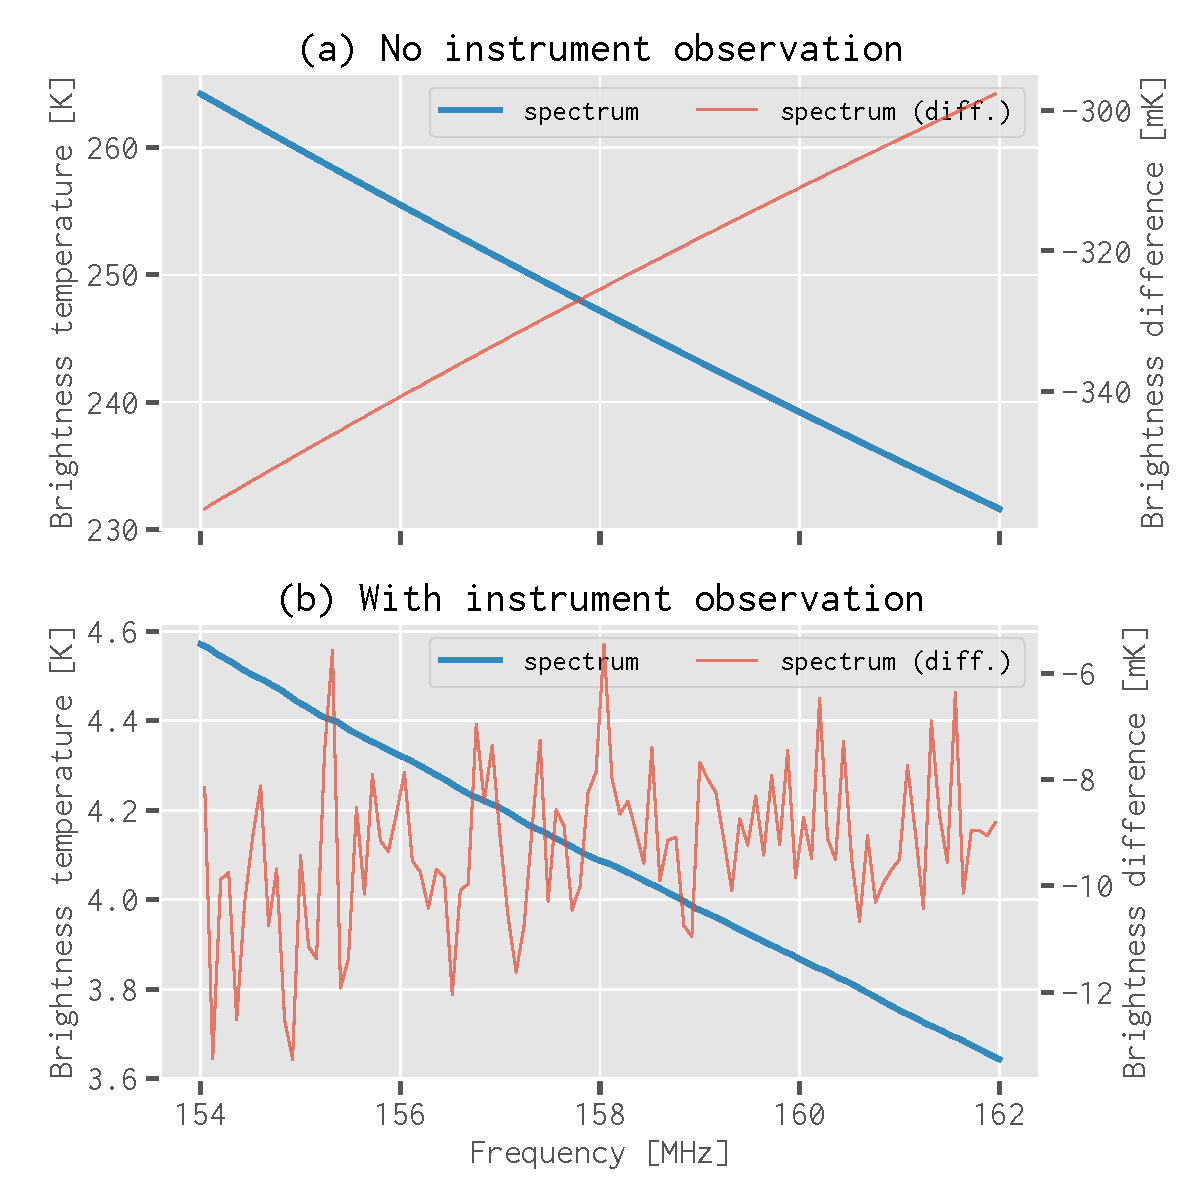
\includegraphics[width=\columnwidth]{simudata}
  \caption{\label{fig:simudata}%
    Example spectra (the bold blue lines) and the corresponding
    differential spectra (the thin red lines) for the foreground
    emission.
    The top and bottom panels show the cases without and with
    instrument observation, respectively.
  }
\end{figure}


%%----------------------------------------------------------------------
\subsection{Data preprocessing}
\label{sec:preprocessing}

The data set $S$ required by the CDAE consists of two parts:
(1) the input data that are the addition of the EoR signal and the
foreground emission, i.e., $X = C_{\R{EoR}} + C_{\R{fg}}$;
(2) the input EoR signal (i.e., $X_{\R{EoR}} = C_{\R{EoR}}$)
that acts as the goal of training the CDAE.

For the input data $X$, we propose to apply the FT along the frequency
dimension, which makes the EoR signal more distinguishable from the
foreground emission and thus easier to learn by the CDAE (see also the
comparison without applying such FT to the data in \autoref{sec:noft}).
The Blackman-Nuttall window function is applied to suppress the
FT side-lobes caused by the sharp discontinuities at the ends
of the finite frequency band \citep[e.g.,][]{chapman2016}.
It is sufficient to keep only half the Fourier coefficients because
the data is real, thus a vector of length 101 representing one pixel in
the image cube is transformed to be 51 complex Fourier coefficients.
We excise the 6 coefficients of the lowest Fourier frequencies, which
have large values and are mostly contributed by the spectral-smooth
foreground emission.
Since both the real and imaginary parts of the Fourier coefficients
are required to reconstruct the frequency-domain signal via inverse FT,
the real and imaginary parts are separated and concatenated into a new
vector of length 90.
Finally, the data are zero-centred and normalised to have unit variance.

The preprocessing steps for the input EoR signal $X_{\R{EoR}}$ are
similar but need minor adjustments.
After applying the FT, excising the 6 lowest Fourier components, and
concatenating the real and imaginary parts,
the elements in the data that have a value less than the 1$^{\R{th}}$
percentile or greater than the 99$^{\R{th}}$ percentile are truncated,
improving the robustness of the data for training the CDAE.
Finally, the data are divided by the maximum absolute value of the
truncated data, constraining the value range to be $[-1, 1]$,
which renders the `tanh' activation function that has the same value
range appropriate for the output layer of the CDAE.


%%----------------------------------------------------------------------
\subsection{Training}
\label{sec:training}

The data set has 129,600 data points, i.e., the number of pixels of
the image cubes, and is randomly partitioned into the
training set ($S_{\R{tr}}$), validation set ($S_{\R{val}}$), and
test set ($S_{\R{test}}$) that account for 60, 20, and 20 per cent of
the whole data set, respectively [这是常用的切分比例].
The training set is used to train the parameters of the CDAE by
minimising the loss,
the validation set helps to determine the hyperparameters (e.g., the
number of layers and filters, the choice of the loss function),
while the test set is only employed to evaluate the performance of the
trained CDAE.

We implement the proposed CDAE using the popular \textsc{Keras}\footnote{%
  Keras: \url{https://keras.io} (version 2.2.0)}
framework \citep{keras} with the \textsc{TensorFlow}\footnote{%
TensorFlow: \url{https://www.tensorflow.org} (version 1.4.1)}
back end \citep{tensorflow} [这是目前最常用的编写神经网络的软件包].
The parameters of the Adam optimisation method are set to the default
values, i.e., learning rate being $\alpha = 0.001$, and
exponential decay rates for the first and second moment estimates being
$\beta_1 = 0.9$ and $\beta_2 = 0.999$, respectively \citep{kingma2015}.
The CDAE is trained on the training set ($S_{\R{tr}}$) with a batch size
of 100 for 100 epochs so that the training loss converges.


%%----------------------------------------------------------------------
\subsection{Results}
\label{sec:results}

The training and validation losses together with the evaluation index
(i.e., the correlation coefficient) calculated on the validation set
($S_{\R{val}}$) during the training phase are shown in \autoref{fig:train}.
The steadily decreasing losses and increasing correlation coefficient
suggest that the CDAE is well trained without overfitting.
By evaluating on the test set ($S_{\R{test}}$), the trained CDAE
achieves excellent performance with a correlation coefficient of
$\rho_{\R{CDAE}} = \num{0.969 +- 0.020}$.
As an example, \autoref{fig:result} illustrates the reconstructed EoR
signal ($\rho = 0.965$) for one random pixel.
Consequently, the proposed CDAE is able to learn the features of the
faint EoR signal and accurately reconstruct it, overcoming the
frequency-dependent beam effects and severe foreground contamination.

\begin{figure}
  \centering
  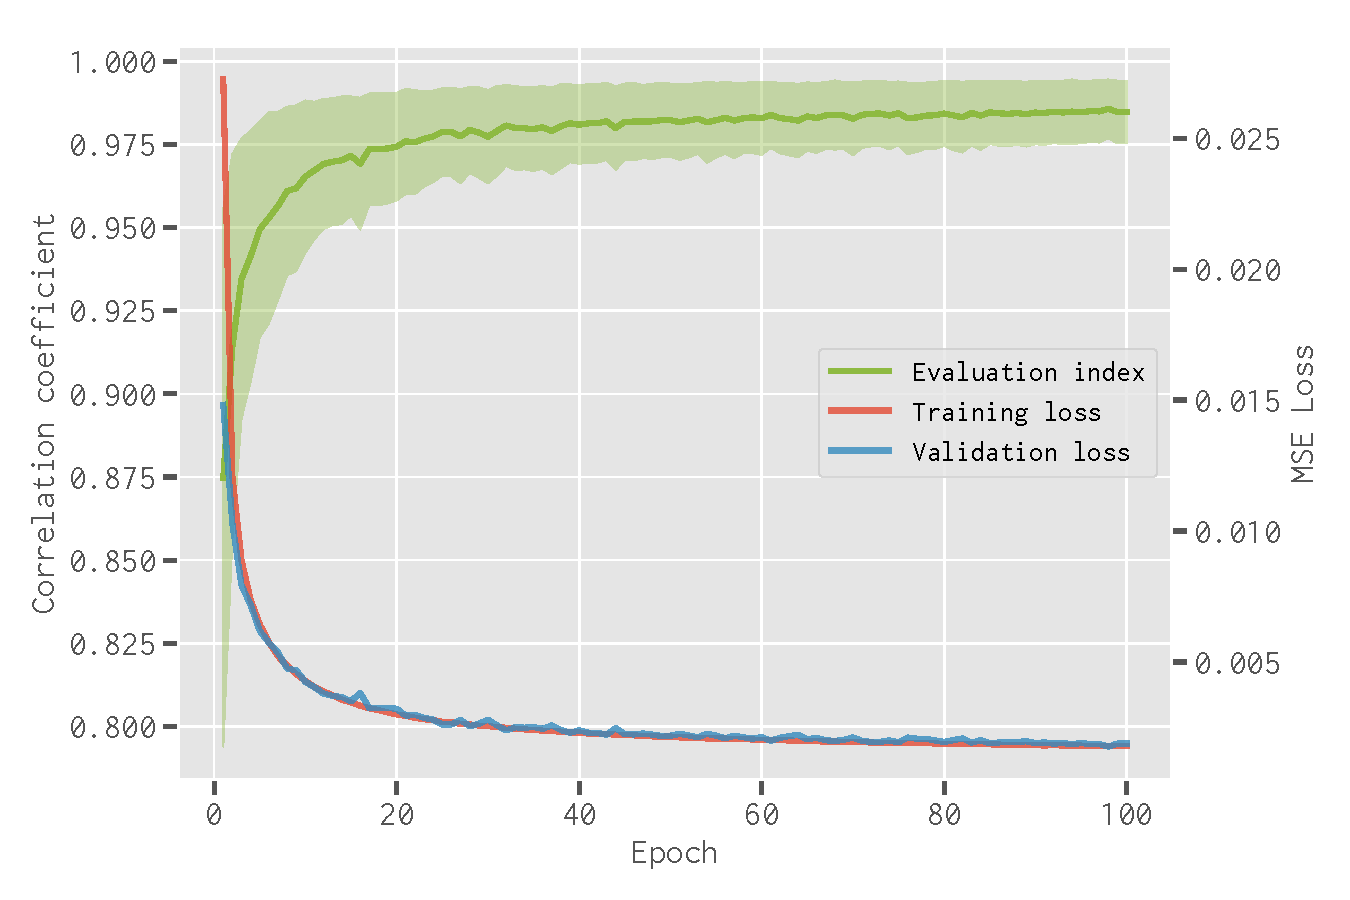
\includegraphics[width=\columnwidth]{cdae-train}
  \caption{\label{fig:train}%
    The training loss (the red line), validation loss (the blue line),
    and correlation coefficient calculated on the validation set
    $S_{\R{val}}$ (the green line with the shaded region representing
    the standard deviation) during the training of the CDAE.
  }
\end{figure}

\begin{figure}
  \centering
  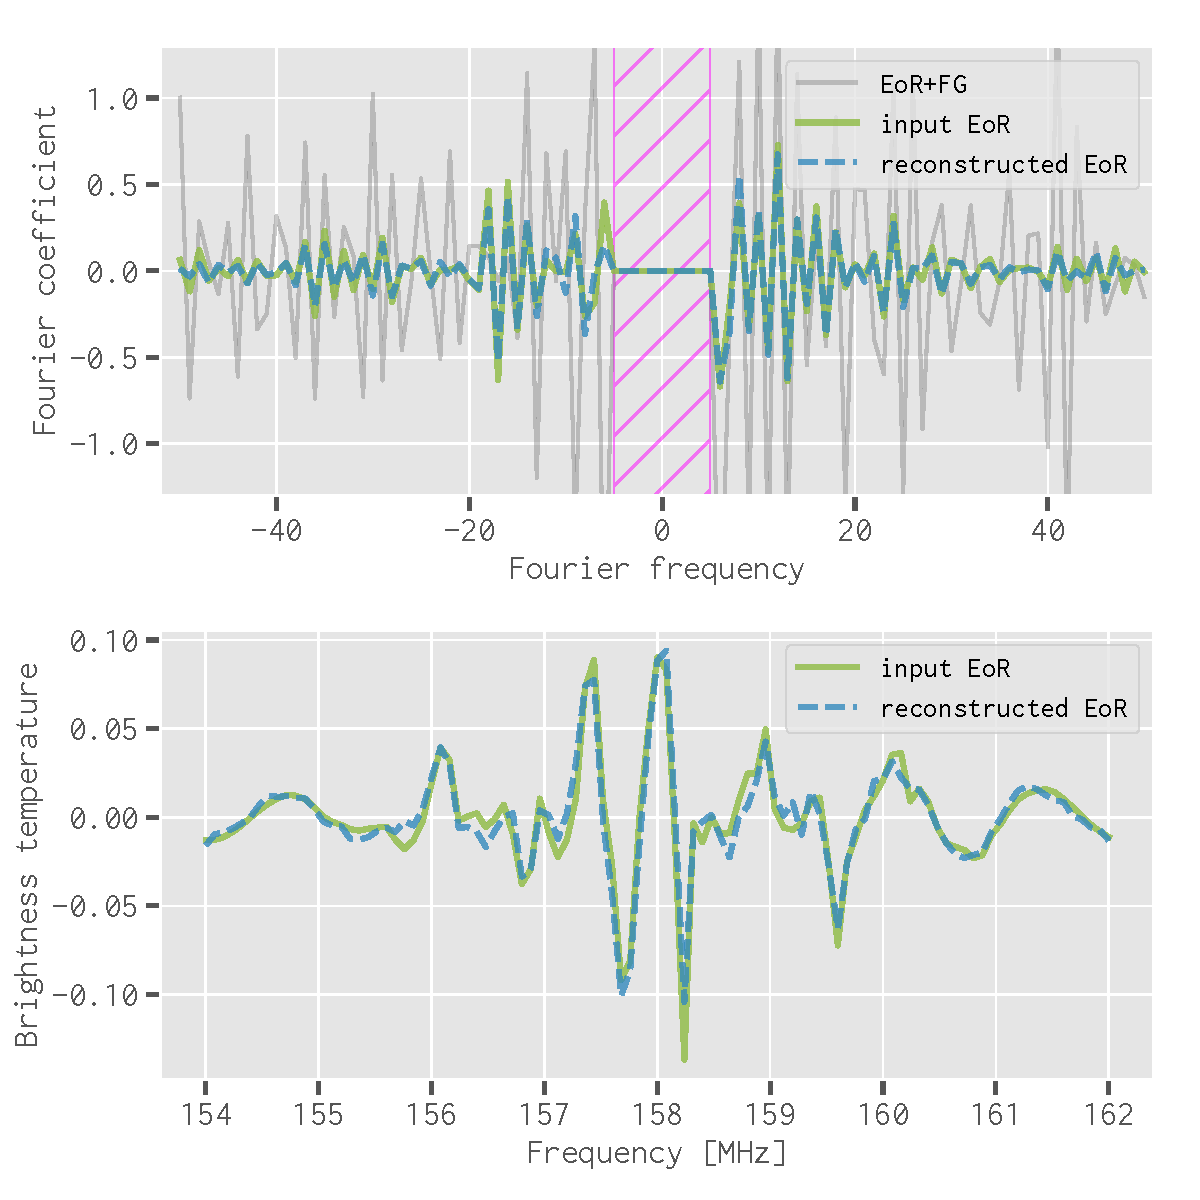
\includegraphics[width=\columnwidth]{eor-result}
  \caption{\label{fig:result}%
    An example of the EoR signal reconstructed by the trained CDAE for
    one random pixel.
    \textbf{(top)} The input EoR signal (the solid green line) and the
    reconstructed EoR signal (the dashed blue line) in the Fourier domain
    where the CDAE training is performed.
    The grey line represents the corresponding input data that are the
    addition of the EoR signal and the foreground emission.
    The magenta hatched region marks the excised Fourier coefficients
    in data preprocessing.
    \textbf{(bottom)} The input EoR signal (the solid green line) and
    the reconstructed EoR signal (the dashed blue line) transformed back
    to the observing frequency domain.
  }
\end{figure}


%%======================================================================
\section{Discussions}
\label{sec:discussions}

%%----------------------------------------------------------------------
\subsection{Without Fourier Transform}
\label{sec:noft}

We perform another experiment using the same CDAE architecture and data,
but the data is preprocessed without applying the FT along the
frequency dimension as depicted in \autoref{sec:preprocessing}.
After training the CDAE in the same way as described in
\autoref{sec:training}, the achieved performance is
$\rho_{\R{noft}} = \num{0.927 +- 0.051}$, which is smaller and has a
larger uncertainty than the case with FT applied, indicating a worse
performance.
The losses and the correlation coefficient on the validation set
during the training phase are presented in \autoref{fig:train-noft}.
We find that the training process is slightly unstable given the small
spikes on the curves of the training loss and the correlation
coefficient.
The training loss also converges slower compared with the case with FT.
Such a comparison indicates that it is beneficial to preprocess the
data by applying the FT along the frequency dimension, because the FT
renders the EoR signal and the foreground emission more distinguishable
in the Fourier domain, where the fluctuating EoR signal concentrates on
larger Fourier modes but the spectral-smooth foreground emission
distributes mainly on smaller Fourier modes.

\begin{figure}
  \centering
  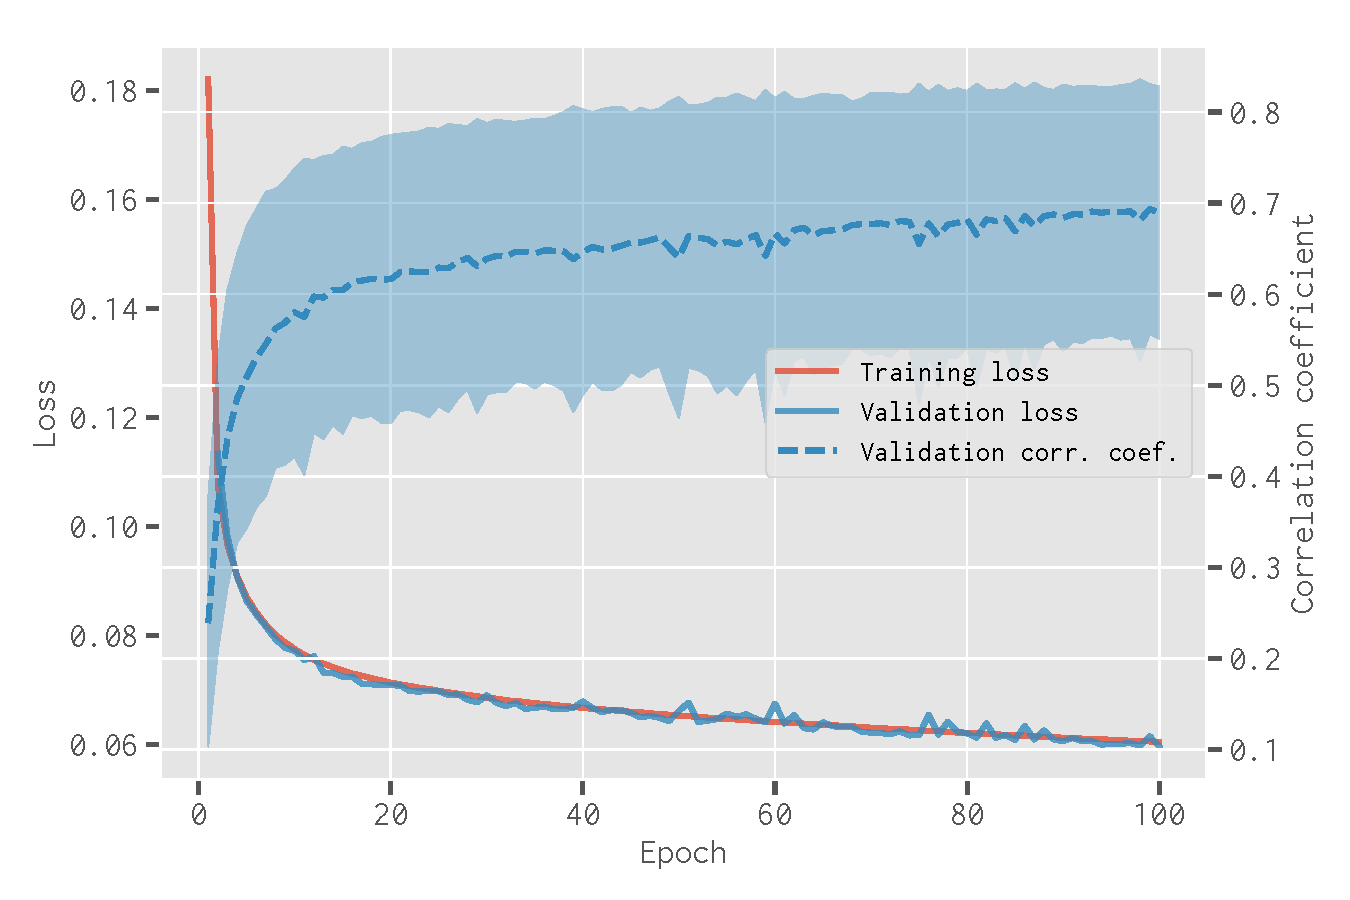
\includegraphics[width=\columnwidth]{cdae-train-noft}
  \caption{\label{fig:train-noft}%
    Same as \autoref{fig:train} but for the case that the data is not
    preprocessed by the FT.
  }
\end{figure}


%%----------------------------------------------------------------------
\subsection{Comparing with polynomial fitting method}
\label{sec:polyfit}

In order to further demonstrate the performance of our method, we carry
out a comparison between our method and the traditional polynomial
fitting method \citep[e.g.,][]{wang2006,liu2009ps}.
Using the same image cubes simulated in \autoref{sec:simulation},
a low-order polynomial is fitted along the frequency dimension for each
pixel in the image cube of the total emission (i.e.,
$C_{\R{tot}} = C_{\R{EoR}} + C_{\R{fg}}$).
Then by subtracting the fitted smooth component, which is regarded as
the foreground emission, the EoR signal is uncovered.
While polynomials of too low order are insufficient to model the
foreground emission, polynomials of too high order risk fitting out
the wanted EoR signal.
We have tested polynomials of order from 2 (quadratic) to 5 (quintic),
and find that the quartic polynomial (order of 4) can give the
relatively best result.
However, the correlation coefficient calculated for the separated EoR
signal in such case is only $\rho_{\R{poly}} = \num{0.241 +- 0.103}$,
which is rather small and indicates that the polynomial fitting method
performs poor in removing the foreground emission.
As illustrated in \autoref{fig:simudata}(b), the frequency-dependent
beam effects cause rapid oscillations, which can be even stronger than
the EoR signal, on the originally smooth foreground spectrum.
The polynomial fitting method, which can only model the smooth
spectrum, is unable to distinguish such rapid oscillations from the
EoR signal, hence leading to poor results.
On the contrary, the proposed CDAE is driven by the data so that it can
learn the differences between the spectra of the EoR signal and the
foreground emission, achieving much better performance.


%%======================================================================
\section{Conclusions}
\label{sec:conclusions}

The frequency-dependent beam effects of radio interferometers can cause
unpredictable and rapid fluctuations along the frequency dimension,
which seriously damage the smoothness of the foreground spectra and
prevent traditional foreground removing methods (e.g., polynomial
fitting) from uncovering the EoR signal.
It is difficult to craft models to overcome such complicated beam
effects, therefore, the data-driven methods, such as the deep learning
methods, that learn from the data seems more feasible and appealing.
To this end, we have proposed a deep-learning-based method by employing
the CDAE to separate the EoR signal.
The CDAE has been trained on the simulated SKA images and achieved
excellent performance in separating the EoR signal, demonstrating its
ability to overcome the intricate frequency-dependent beam effects.
In addition, the proposed CDAE has a simple architecture and is easily
extensible, exhibiting the great potential of deep learning methods
to play an important role in the forthcoming EoR experiments.


%%======================================================================
\section*{Acknowledgements}

We would like to thank Jeffrey Hsu for reading the manuscript and
providing suggestions.
This work is supported by
the Ministry of Science and Technology of China
(grant Nos. 2018YFA0404601, 2017YFF0210903),
and the National Natural Science Foundation of China
(grant Nos. 11433002, 11621303, 11835009, 61371147).


%%======================================================================
%% References

\bibliographystyle{mnras}
\bibliography{references}


%%======================================================================
%% Appendix

% \appendix


%%======================================================================
% Don't change these lines
\bsp	% typesetting comment
\label{lastpage}
\end{document}

%% EOF
